%-------------------------------------------------------------------------------
% seq64_patterns_panel
%-------------------------------------------------------------------------------
%
% \file        seq64_patterns_panel.tex
% \library     Documents
% \author      Chris Ahlstrom
% \date        2015-08-31
% \update      2016-10-21
% \version     $Revision$
% \license     $XPC_GPL_LICENSE$
%
%     Provides the concepts.
%
%-------------------------------------------------------------------------------

\section{Patterns Panel}
\label{sec:seq64_patterns_panel}

   \textsl{Sequencer64} works with the idea of patterns (loops) that are
   repeated all along a song.  One composes and edits small patterns, and
   combines them to create a full song.  This is a powerful way to work, and
   makes one productive within an hour.

   The \textsl{Sequencer64 Patterns Panel} is the main window of
   \textsl{Sequencer64}.
   See \figureref{fig:seq64_main_screen}.
   It is also called the "main window" or the "patterns window".
   It is here one creates a set of patterns
   (see \sectionref{subsubsec:concepts_terms_screen_set}),
   manages the configuration, and opens the pattern or song editors.

   \index{live mode}
   \index{mode!live}
   \index{mode!ALSA}
   When the Patterns Panel has the application focus (in ALSA mode),
   and \textsl{Sequencer64}
   is \textsl{not} running in JACK mode, it puts
   \textsl{Sequencer64} in "live mode".  The musician can
   control the playback and muting/unmuting of each pattern in
   the song, while it is playing, from within this window.

   \index{song mode}
   \index{mode!song}
   \index{mode!ALSA}
   If the song editor
   (see \sectionref{sec:seq64_song_editor})
   has the input focus in ALSA mode, then it controls the muting/unmuting of
   each pattern, and \textsl{Sequencer64} runs in "song mode".

   However, if \textsl{Sequencer64} is using JACK transport, then, instead of
   the behavior described above, live versus song mode is controlled by the
   JACK start mode option (see the \textbf{JACK Start mode} item in
   \sectionref{paragraph:seq64_menu_file_options_jack_sync}).

   Back to the patterns panel....  For exposition, we break the Patterns Panel
   into a menu bar, a top panel, a pattern panel, and a bottom panel.  (Note
   that the \textsl{Sequencer64} menu bar was already discussed in
   \sectionref{sec:seq64_menu}.)

\subsection{Patterns / Top Panel}
\label{subsec:seq64_patterns_panel_top}

   The top panel of the Pattern window is simple, consisting of the name of
   the program and a couple of controls.  The original version looked like
   this:

\begin{figure}[H]
   \centering 
   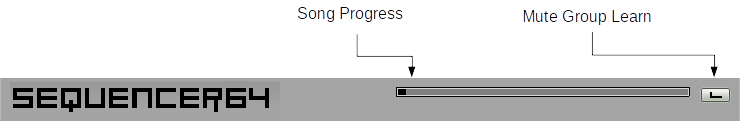
\includegraphics[scale=0.75]{pattern-window-top-panel-items.png}
   \caption{Patterns Panel, Top Panel, Older Version}
   \label{fig:pattern_window_top_panel_items}
\end{figure}

   But, if compiled with \texttt{SEQ64\_STAZED\_MENU\_BUTTONS} defined,
   there are some extra buttons available:

\begin{figure}[H]
   \centering 
   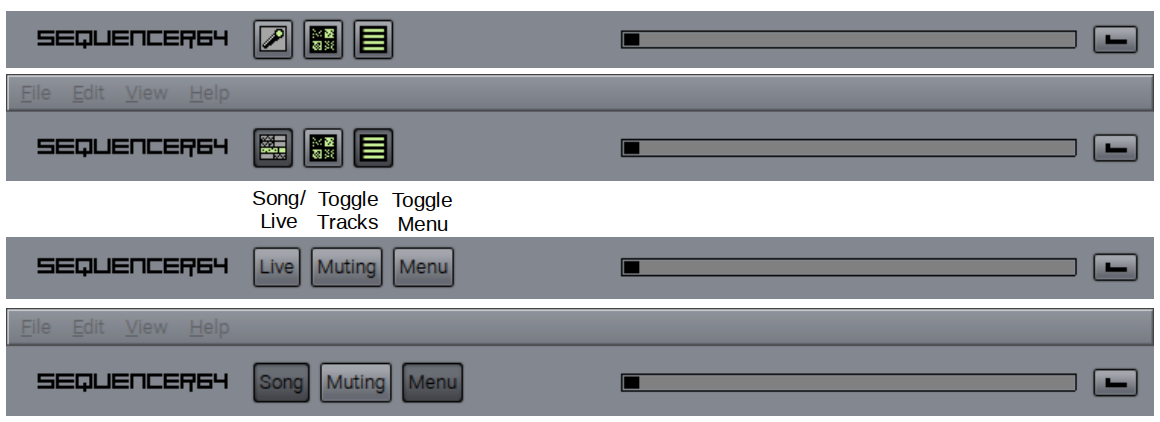
\includegraphics[scale=0.50]{pattern-window-top-panel-items-new.png}
   \caption{Patterns Panel, New Top Panel Items}
   \label{fig:pattern_window_new_top_panel_items}
\end{figure}

   This figure shows the possible appearance of the main window top panel.
   If \textsl{Sequencer64} was built with
   \texttt{SEQ64\_MENU\_BUTTON\_PIXMAPS} defined, then the buttons have icons
   on them; otherwise they have text.  The figure shows what they look like,
   and how they look with the song/live and toggle-menu functions activated.
 
   \begin{enumber}
      \item \textbf{Song/Live}
      \item \textbf{Toggle Tracks}
      \item \textbf{Toggle Menu}
      \item \textbf{Song Progress}
      \item \textbf{Mute Group Learn}
   \end{enumber}

   \setcounter{ItemCounter}{0}      % Reset the ItemCounter for this list.

   \itempar{Song/Live}{pattern!song/live}
   \index{song!song/live}
   This new button allows the Song mode to be in force even if
   the \textbf{Song Editor} does not have the focus of the application.
   However, if the \textbf{Song Editor} does have focus, it overrides this
   button, to preserve expected behavior.
   There is also a configurable hotkey associated with it,
   which defaults to \texttt{F1}, and is configurable in the "rc" file and
   the \textbf{File / Options / Ext Keys} page.

   \itempar{Toggle Tracks}{pattern!toggle tracks}
   \index{song!toggle tracks}
   This button changes the status of all of the tracks, reversing the mute
   status of each pattern.
   There is also a configurable hotkey associated with it, called
   \textbf{Toggle mutes},
   which defaults to \texttt{F8}, and is configurable in the "rc" file and
   the \textbf{File / Options / Ext Keys} page.

   \itempar{Toggle Menu}{pattern!toggle menu}
   \index{song!toggle menu}
   This button enables and disables the main menu of the main window.
   Disabling it allows additional hotkeys to be used without calling forth menu
   entries.
   There is also a configurable hotkey associated with it, called
   \textbf{Menu mode},
   which defaults to \texttt{F3}, and is configurable in the "rc" file and
   the \textbf{File / Options / Ext Keys} page.

   \itempar{Song Progress}{pattern!progress}
   \index{song!progress}
   \index{song!"main time"}
   The \textbf{Song Progress} bar is also known as the "main time" bar.
   This bar shows a number of small black cursors ("pills") that show the
   progress of the song through the various patterns.  For short patterns,
   the progress is fast.  For patterns that last longer, the progress is
   slow.  The whole field flashes in time with the beat.
   This field shows that something is going on.  It can also indicate
   the relative lengths of the various patterns.
 
   Note that the individual pattern boxes in the main panel, for
   patterns that are not empty, have their own
   moving progress cursor, a vertical line in each box.
   By default, this progress line is black, but it can be changed to
   other colors via a "user" configuration file entry in the 
   \texttt{[user-interface-settings]} section.
   Set the \texttt{progress\_bar\_colored} item to a value ranging from 0
   (black) to 6 (dark cyan).
   There is also a \texttt{progress\_bar\_thick} item to enable a thicker
   progress bar, for better visibility.

%  Even if not enabled, the currently-selected pattern will show as highlighted
%  in dark-cyan.

   \itempar{Mute Group Learn}{pattern!mute group learn}
   \index{L button}
   \index{"L" button}
   This button is also known as the "L" button.
   Click this button, and then press a mute-group key
   to store the mute-state (whether armed or unarmed)
   of all the patterns with in that key.
   In addition to clicking this button, one can also press
   the \texttt{Ctrl-L} combination (analogous to the \texttt{Ctrl-E}
   keystroke that brings up the Song Editor).
   \index{auto-shift}
   \index{group-learn!auto-shift}
   When in group-learn mode, the \texttt{Shift} key cannot be hit, so the
   group-learn mode automatically converts the keys to their shifted versions.
   \index{shift-lock}
   \index{group-learn!shift-lock}
   This feature known as \textsl{shift-lock} or \textsl{auto-shift}.

   See the \textbf{File / Options / Keyboard} menu entry to bring up the
   dialog showing the available mute-group keys and the corresponding
   hot-key for the "L" button.
   This key is usually the \texttt{Insert} key.  Unlike the button or the
   \texttt{Ctrl-L} key, this key must be held down while pressing the desired
   mute-group key.
   This is a clumsy thing on our main keyboard... one must press and hold
   \texttt{Shift-Fn-Insert} to get the \texttt{Insert} key, and then also
   press the desired mute-group key.  A real knuckle-buster!
   We have our own alternate setup (stored in the file
   \texttt{sequencer64.rc.example}.
   And we've also added the "shift-lock" feature for this reason.

   Group-learn is a modifier key to be pressed
%  \textsl{together} with
   just before pressing
   the desired group key, and the group on/off keys are there to enable
   each group, \textsl{not} to toggle group states.

   To set up the mute groups, press the 'L' button, and then press a key on
   the keyboard to 'learn' or 'save' the preset. Looking at the list of keys
   assigned for these mute groups (in \textbf{File / Options / Keyboard}),
   the first bank of keys are "!", "'", "?", etc., and the second bank are
   "Q", "W" "E", etc.  Note that these keys do not toggle patterns, but simply
   turn them on (they unmute them, i.e. arm them).
   If the key is valid, then the following prompt occurs:

\begin{figure}[H]
   \centering 
   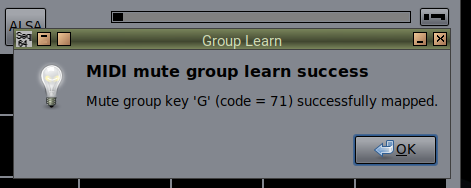
\includegraphics[scale=1.0]{pattern-window-group-learn-confirmation.png}
   \caption{Group Learn Confirmation Prompt}
   \label{fig:pattern_window_group_learn_confirmation}
\end{figure}
   
   When you ask the program to 'learn' the key, one cannot
   use the Shift key, so one normally could not use the "!" or
   other symbol keys.
   In fact, the process stops as soon as the Shift key is pressed:

\begin{figure}[H]
   \centering 
   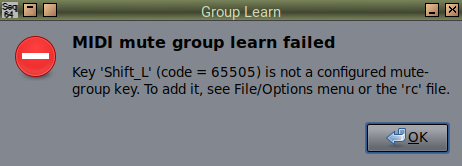
\includegraphics[scale=1.0]{pattern-window-group-learn-failure.png}
   \caption{Group Learn Failure Prompt (Shift Key)}
   \label{fig:pattern_window_group_learn_failure}
\end{figure}

   \textbf{New:}
   \index{new!caps lock in learn mode}
   To avoid this issue with the Shift key, \textsl{Sequencer64} now
   "Shift-Locks" the keys for you, so that none of the keys, whether letters or
   the punctuation characters above the numbers, need the Shift key to be held.
   There is now no need to use the \textbf{Caps Lock} is \textsl{On} before
   starting the 'learn' process.  We did this because we tend to map the
   \texttt{Caps Lock} key as the \textsl{true} Control key, so that
   \texttt{Caps Lock} is no longer available... it is one of the most useless
   keys every.

   Once that works, one can configure the MIDI settings in similar ways
   by assigning MIDI commands to arm or toggle loops, using 
   \index{rc file}
   the 'on' option in the "rc" file.
   See \sectionref{subsec:seq64_rc_file_midi_control}.

%  The mute group doesn't toggle... it turns on.
%  \index{group!toggle}
   \index{group!arm}
   \index{group!unmute}
%  One can toggle the playing status of up to 32 previously
   One can set the playing status of up to 32 previously
   defined mute/unmute patterns (groups) in the active screenset, similar to
   hardware sequencers.  One can mute-unmute (according to the group
   definition) all loops in the playing screenset, which is the only one that
   can have sequences playing if a mute group is selected
   (like a live sequencer).

   This arming is done either by one of the \textsl{group arm} keys
   or by a MIDI controller, both assigned in the
   \index{rc file}
   \texttt{~/.config/sequencer64/sequencer64.rc} or \texttt{~/.seq24rc} files,
   and easily modified in the \textbf{File / Options / Keyboard} tab.
   These characters can be shown in each pattern (and in 0.9.11 and above, no
   matter which screenset is active).

   A mute/unmute pattern (group) is stored by holding a
   \index{group!learn}
   \textsl{group learn} key (\texttt{Insert} by default) while pressing the
   corresponding \textsl{group arm} key.
   There are also keys assigned to turn on/off the group functionality.

   Remember that groups work with the playing ("in-view") screen set.
   One must change the screenset and give it the command to make it the
   playing one
   \index{keys!Home}
   (some set the \texttt{Home} key for this purpose).
   So, for example, if one sets \texttt{A} to turn on the
   patterns in slots 1 and 2 in set 0 (the first set), then pressing
   \texttt{A} in another set will arm the patterns in the same relative
   location in that set.
   This setup is flexible, but takes some thought.
   One can set up a number of mute-groups, and decide to use them
   for all sets, or mentally allocate one mute-group per set.
   Please note that a mute-group key does \textsl{toggle} the saved
   armed patterns... it can only turn them on.

   \index{rc file}
   Everything is configurable in the "rc" file.

\subsection{Patterns / Main Panel}
\label{subsec:seq64_patterns_panel_main}

   The main panel of the Patterns window provides a grid of empty boxes,
   each box delimited by brace-like lines at left and right.
   Each filled box represents a loop or pattern.
   One sees only 32 loops at a time in the main panel (but many more than
   32 loops can be supported by \textsl{Sequencer64}).
   \index{screen set}
   This group of 32 loops is called a "screen set", as discussed in
   \sectionref{subsubsec:concepts_terms_screen_set}.
   One can switch between sets by using the
   \index{keys![}
   \texttt{[} and
   \index{keys!]}
   \texttt{]} keys on the keyboard, or by using
   the spin-widget-driven, labelled \textbf{Set} interface item, or
   \index{keys!Home}
   by hitting the (default) Home key to make it the playing screenset.
   There are a total of 32 sets, for a total of 1024 loops/patterns. 
   Only one screen set can be playing at a time, according to other notes we
   have found.  Have not yet tried to verify this assertion.

\begin{figure}[H]
   \centering 
   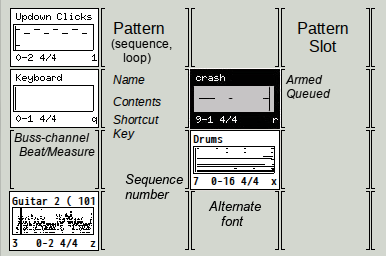
\includegraphics[scale=0.75]{pattern-window-main-panel-items.png}
   \caption{Patterns Panel, Main Panel Items}
   \label{fig:pattern_window_main_panel_items}
\end{figure}

   The individual items annoted in this figure are described in
   \sectionref{subsubsec:seq64_patterns_pattern_filled}, in more detail.
   \textbf{However}, this figure does not show the new feature where the
   sequence number appears at the bottom left of the slot.  Observe that
   feature in the first figure of the next section.

   \begin{enumber}
      \item \textbf{Pattern Slot}
      \item \textbf{Pattern}
   \end{enumber}

\subsubsection{Pattern Slot}
\label{subsubsec:seq64_patterns_pattern_slot}

   \index{pattern!slot}
   An empty box is a slot for a pattern.

   A pattern slot can show a number of different statuses based on the coloring
   of elements in the slot. 

\begin{figure}[H]
   \centering 
   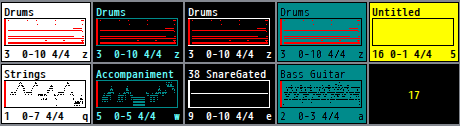
\includegraphics[scale=0.75]{new/slots.png}
   \caption{Various Status of Pattern Slots}
   \label{fig:pattern_slots_statuses}
\end{figure}

   The colors have meaning:

   \begin{itemize}
      \item \textbf{Empty background}.  Whether the classic gray pattern
         of \textsl{Seq24}, or the many patterns of \textsl{Sequencer64},
         including all black with yellow sequence numbers, this
         slot coloring indicates that it is unused.
      \item \textbf{White background}.  Unarmed (muted) pattern.
      \item \textbf{Black background}.  Armed (unmuted) pattern.  If the text
      is yellow, it is a pattern with no MIDI events, but is armed.
      Note that armed/unmuted patterns can be exported if they have a layout
      in the Song Editor.
      \item \textbf{Yellow background}.  A pattern with no MIDI events, just
         textual MIDI information.
      \item \textbf{Cyan background, black text}.
         An unarmed pattern currently being edited in a pattern editor or event
         editor. Or, if an SMF 0 MIDI file was just opened or imported, this
         color combination indicates the SMF 0 format track with all of the
         data in the song.
      \item \textbf{Black background, cyan text}.
         An armed pattern currently being edited in a pattern editor or event
         editor.  Or an armed SMF 0 format MIDI sequence.
      \item \textbf{Red events}.
         Indicates a pattern for which the new transpose feature is
         disabled.  The white, black, and cyan background have the same
         meanings as in the other items for statuses of unarmed, armed, and
         currently being edited.
   \end{itemize}

   \index{pattern!right click}
   \index{slot!empty slot right-click}
   By right-clicking on an empty box one brings up a menu to create
   a new loop, as well as some other operations:

\begin{figure}[H]
   \centering 
   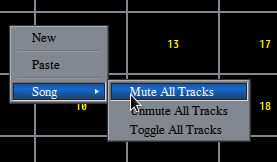
\includegraphics[scale=0.75]{pattern/pattern-empty-right-click-menu.png}
   \caption{Empty Pattern, Right-Click Menu}
   \label{fig:pattern_window_empty_right_click}
\end{figure}

   \begin{enumber}
      \item \textbf{New}
      \item \textbf{Paste}
      \item \textbf{Song}
      \begin{itemize}
         \item {Mute All Tracks}
         \item {Unmute All Tracks}
         \item {Toggle All Tracks}
      \end{itemize}
   \end{enumber}

   \setcounter{ItemCounter}{0}      % Reset the ItemCounter for this list.

   \itempar{New}{pattern!new}
   Creates a new loop or pattern.
   Clicking this menu entry fills in the empty box with an untitled
   pattern, and brings up the Pattern Editor
   so that one can fill in the new pattern.

   In addition to right-clicking and selecting \textbf{New}, the user can
   \index{new!empty slot double-click}
   double-click on the empty slot, to bring up a new instance of the sequence
   editor.  For the double-click, the effect can be a bit confusing at first,
   because it currently also toggles the arming/mute status of the slot
   quickly twice (leaving it as it was), as well.  It might take some getting
   used to, but we miss it when using \textsl{Seq24}.

   \index{new!editing shortcut}
   \index{keys!=}
   \index{keys!-}
   An new feature is hitting the equals ("=") key, then hitting
   a shortcut key (hotkey), to bring up a new sequence or edit an existing one
   in a pattern editor.  Another new feature is hitting the minus ("-") key,
   then the hotkey, to bring up the event editor.
   We do not yet have a user-interface and
   configuration file settings for the the '=' and '-' keys.
   We would still like a way to edit sequences without requiring a mouse!

   \index{new!current slot highlight}
   When an unarmed (muted) pattern is first brough up for sequence editing (or
   event editing), the slot in the main window is now highlighted, using black
   text on a cyan background, as being the "currently-edited" slot.
   (This is the same background used to indicate the original track in an
   SMF 0 to SMF 1 conversion.)

\begin{figure}[H]
   \centering 
   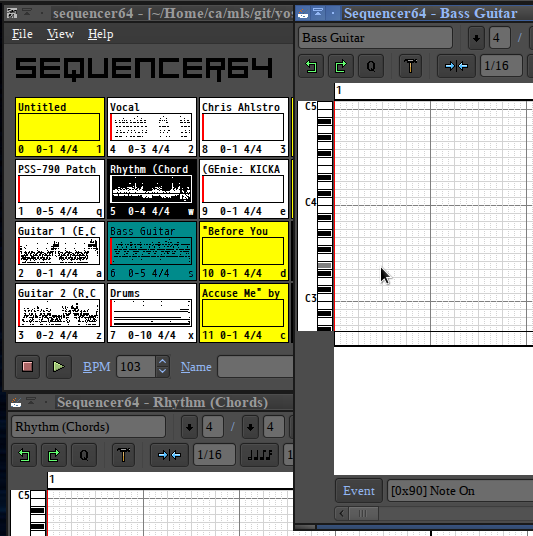
\includegraphics[scale=0.75]{pattern-window-current-seq-unarmed.png}
   \caption{Currently-Edited Pattern, Unarmed}
   \label{fig:pattern_window_current_seq_unarmed}
\end{figure}

   If the currently-edited sequence is armed (unmuted), then the highlighting
   is reversed (cyan text on a black background), and resembles the
   highlighting for an armed sequence (which is white text on a black
   background).

\begin{figure}[H]
   \centering 
   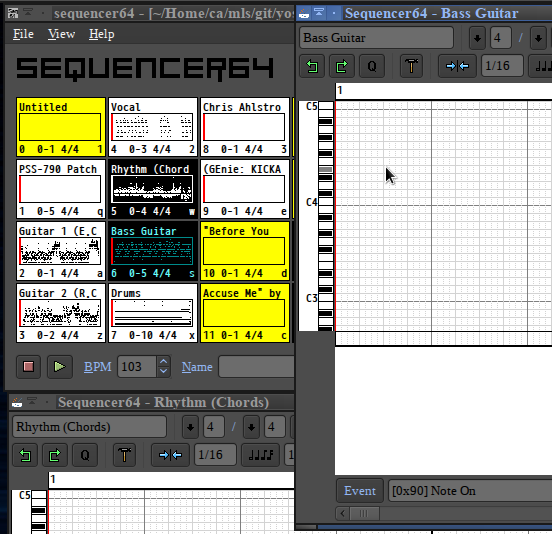
\includegraphics[scale=0.75]{pattern-window-current-seq-armed.png}
   \caption{Currently-Edited Pattern, Armed}
   \label{fig:pattern_window_current_seq_armed}
\end{figure}

   If more than one sequence or event editor is brought up, only the slot for
   the last one to have focus is hightlighted.
   Note that this highlighting also applies to the (new) Event Editor.

   \itempar{Paste}{pattern!paste}
   Pastes a loop or pattern that was previously copied.

   \itempar{Song / Mute All Tracks}{pattern!mute all}
   This item mutes all tracks (or loops/patterns).
   It works when one has opened the Song Editor window
   and started playing in playback
   mode by starting play using that window.

   So, let us assume the song is running in playback mode.  The patterns that
   are active (unmuted) in by that playback window are shown with a black
   background in the main patterns window.  If one right clicks on a pattern
   cell and selects \textbf{Song / Mute All Tracks}, all those patterns
   will become white and be silenced.  Eventually, the Song Editor window
   catches up and shows the "M" activated for all tracks.

   \itempar{Song / Unmute All Tracks}{pattern!unmute all}
   Provides the opposite functionality, making all tracks armed and audible.

   \itempar{Song / Toggle All Tracks}{pattern!toggle mute all}
   Toggles the armed/mute status of all tracks.

   Note that there is also a feature where a
   \texttt{Shift-Left-Click} on a pattern slot toggles the mute
   status of all of the other \textsl{tracks}.
   
\subsubsection{Pattern}
\label{subsubsec:seq64_patterns_pattern_filled}

   A filled pattern slot is referred to informally as a pattern.
   A pattern is shown in the Pattern windows as a filled box with the
   following items of information in it.
   Examine \figureref{fig:pattern_window_main_panel_items}; it shows
   these items annotated for clarity.

   \begin{itemize}
      \item \textbf{Name}.
         \index{pattern!name}
         This line contains the name or title of the pattern, to help
         reference it when juggling a number of patters.
      \item \textbf{Contents}.
         \index{pattern!contents}
         The contents of the pattern provide a fairly detailed and
         distinguishable representation of the notes or events in the
         pattern.  Also, when the song is playing, a vertical bar cursor
         tracks the position of the playback of the pattern or loop; it
         returns to the beginning of the box every time that pattern starts
         over again.
         \textbf{New:}
         \index{new!empty pattern}
         With \textsl{Sequencer64}, an imported empty pattern will no longer
         needlessly scroll.
         However, if a pattern has even a single event (say, a program change),
         it will scroll.
         \textbf{TODO:}
         \index{todo:one-shot pattern}
         It might be good to have some patterns marked as one-shot patterns.
         They play once at the start of playback, and that is it.
         They could be marked with a cyan background.
         Currently, it is easy enough to use the Song Editor for this purpose,
         but then one cannot play the patterns in live mode.
      \item \textbf{Sequence Number}.
         If the option to show the sequencer number is set
         in the \textbf{File / Options / Keyboard} section
         (see \sectionref{paragraph:seq64_menu_file_options_keyboard},
         the this number is shown at the bottom left of the pattern slot.
      \item \textbf{Bus-Channel}.
         \index{pattern!bus-channel}
         This pair of numbers shows the the MIDI buss number, a dash, and
         the MIDI channel number.
         For example, "0-2" means MIDI buss 0, channel 2.
      \item \textbf{Beat}.
         \index{pattern!beat}
         This pair of numbers is the standard time-signature of the pattern,
         such as "4/4" or "3/4".  The first number is the beats-per-measure,
         and the second is the size of the beat, here, a quarter note.
      \item \textbf{Shortcut Key}.
         If the display of shortcut keys is enabled (see
         \sectionref{paragraph:seq64_menu_file_options_keyboard}),
         then the key noted in the lower-right corner of the pattern can be
         pressed to toggle the mute/unmute status of that pattern.
         This action is an alternative to left-clicking on the pattern.
      \item \textbf{Progress Cursor}.
         At the left of each box is a vertical line, waiting for playback to
         start so that it can move through the pattern, again and again.
      \item \textbf{Armed}.
         See \figureref{fig:pattern_window_main_panel_items}; it shows a black
         and white pattern.  The black color indicates that the pattern is armed
         (unmuted), and will play if playback is initiated in the pattern
         \index{live mode}
         window in live mode.
         An item is armed/disarmed by left-clicking on it.
         \index{shift left click}
         If the Shift key is held while left-clicking on a pattern, then
         the armed/unarmed state of every other active pattern is toggled.
         This feature is useful for isolating a single track or pattern.
      \item \textbf{Queued}.
         That same pattern also shows that it is queued, which means that it
         will start playing when the pattern next begins again.
      \item \textbf{Alternate font}.
         Later builds of \textsl{Sequencer64} are now built with a new font.
         See \figureref{fig:pattern_window_main_panel_items}.  It shows the new
         font. 
         The old font can be selected in the "user" configuration file, and is
         also selected automatically if \textsl{Sequencer64} is run in the
         \textsl{legacy} mode.
      \item \textbf{Sequence number}.
         Later builds of \textsl{Sequencer64} are now built with the option to
         also show the sequence number in the pattern box, if the "show
         sequence numbers" option is on.
         This option can be set in the "user" configuration file.
         See \figureref{fig:pattern_window_main_panel_items}.  It shows an
         example of the sequence number, using the new font.
   \end{itemize}

   \index{pattern!left click}
   Left-clicking on an filled pattern box will toggle the status of the
   pattern between muted (white background) and unmuted (black background).
   If the song is playing via the main window, toggling this status makes
   the pattern stop playing or start playing.  Note that the armed status
   can also be toggled using hot-keys.

   Also note that, if the Song Editor is the active window and was used to
   start the playback, the pattern boxes will toggle between the muted/unmuted
   states as the music plays, and the pattern is active or inactive at the
   point of playback.  (The Song Editor acts as a list of triggers).

   \index{pattern!right click}
   By right-clicking on an already-filled box, one brings up a menu
   to allow one to edit a existing one, or perform a few other actions
   specified in the context menu.  Here is that menu:

\begin{figure}[H]
   \centering 
%  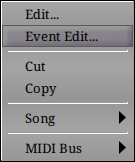
\includegraphics[scale=0.75]{pattern/pattern-right-click-menu.png}
   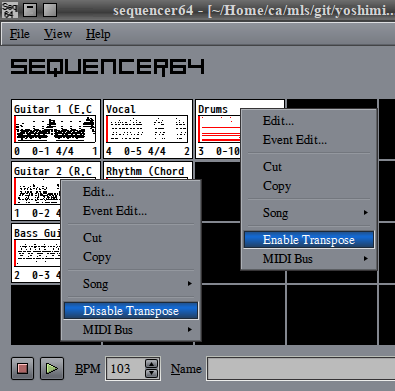
\includegraphics[scale=0.75]{new/seqmenu-menus-0_9_15.png}
   \caption{Existing Pattern, Right-Click Menus}
   \label{fig:pattern_window_right_click}
\end{figure}

   Here one can choose to edit the pattern, cut and copy the pattern,
   set the MIDI bus/channel, and more.
   One can also clear all performance data for the pattern.
   
   \begin{enumber}
      \item \textbf{Edit...}
      \item \textbf{Event Edit...}
      \item \textbf{Cut}
      \item \textbf{Copy}
      \item \textbf{Song/}
      \item \textbf{Enable or Disable Transpose/}
      \item \textbf{MIDI Bus/}
   \end{enumber}

   \setcounter{ItemCounter}{0}      % Reset the ItemCounter for this list.

   \itempar{Edit...}{pattern!edit}
   Edits an existing loop or pattern.
   Clicking this menu entry brings up the \textbf{Pattern Editor}
   so that one can modify the existing pattern by click-dragging new notes in a
   piano roll user-interface.
   See \figureref{fig:pattern_edit_window}.
   Also known as the "sequence editor".

   \textbf{New:}
   In addition to right-clicking and selecting \textbf{Edit...}, the user can
   \index{new!empty slot double-click}
   double-click on the empty slot, to bring up the sequence editor.

   \textbf{New:}
   \index{new!pattern =}
   \index{keys!=}
   Another way to bring up a pattern in the pattern editor is to
   click the \textbf{equal} key and then the pattern's shortcut key.
   For example, "\textbf{= q}" will open up the editor for that pattern.
   Currently, the equals key is hard-wired as the key that does this action.

   \itempar{Event Edit...}{pattern!event edit}
   \textbf{New:}
   \index{new!pattern event edit}
   Edits an existing loop or pattern, but using a detailed event editor that
   shows events as text and numbers, and allows editing them as text and
   numbers.
   Clicking this menu entry brings up the \textbf{Event Editor}
   so that one can view and modify the events in the existing pattern.
   See \figureref{fig:pattern_edit_window}.

   \textbf{New:}
   \index{new!pattern -}
   \index{keys!-}
   Another way to bring up a pattern in the event editor is to
   click the \textbf{minus} key and then the pattern's shortcut key.
   For example, "\textbf{- q}" will open up the event editor for that pattern.
   Currently, the minus key is hard-wired as the key that does this action.

   There are two things to note about this editor.
   First, this editor is not the same as the event editor pane in the pattern
   editor -- it shows all events at once, and shows them only in text format.
   Second, this editor is still a work in progress.
   See \sectionref{sec:seq64_event_editor}, for more information.

   Now, in order to simplify the application, and avoid editing a pattern in
   two different dialogs, if either the pattern editor or the event editor is
   active for a given seqeuence, the right-click sequence-slot menu leaves out
   the \textbf{Edit...} and \textbf{Event Edit...} menu entries.
   This trimmed menu looks like this:

\begin{figure}[H]
   \centering 
   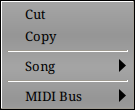
\includegraphics[scale=0.75]{pattern/pattern-right-click-menu-no-edit.png}
   \caption{Existing Pattern, Right-Click Menu Without Edit Entries}
   \label{fig:pattern_window_right_click_no_edit}
\end{figure}

   The old functionality was to have the \textbf{Edit...} menu entry simply
   raise the existing pattern editor to the top of the windows.

   \itempar{Cut}{pattern!cut}
   Deletes and copies an existing loop or pattern.
   Note than one can also drag-and-drop a pattern into another cell.
   \textbf{Bug:}
   \index{bugs!pattern cut not dirty}
   Although this operation works, it does not cause the user to be prompted if
   the application is exited.

   \itempar{Copy}{pattern!copy}
   Copies an existing loop or pattern.
   The pattern can then be pasted elsewhere in the Patterns panel.
   See \sectionref{subsubsec:seq64_patterns_pattern_slot}.

   \itempar{Song}{pattern!song}
   Clicking this menu entry brings up a small popup menu:

\begin{figure}[H]
   \centering 
%  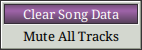
\includegraphics[scale=0.75]{pattern/pattern-menu-song.png}
   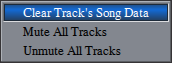
\includegraphics[scale=0.75]{new/seqmenu_song_menu-0_9_15.png}
   \caption{Existing Pattern, Right-Click Menu, Song}
   \label{fig:pattern_window_right_click_song}
\end{figure}

   \begin{enumber}
      \item \textbf{Clear Track's Song Data}
      \item \textbf{Mute All Tracks}
      \item \textbf{Unmute All Tracks}
   \end{enumber}

   \setcounter{ItemCounter}{0}      % Reset the ItemCounter for this list.

   \itempar{Clear Track's Song Data}{pattern!clear song data}
   Selecting this filled-box right-click menu item causes that box's
   loop/pattern to be removed from the song.  This means
   that it disappears from the Song Editor window, and so will not
   be played when the song plays in Song mode.

   \itempar{Mute All Tracks}{pattern!mute all tracks}
   Selecting this filled-box right-click menu item causes
   the tracks in the Song Editor to be muted.  Sometime it takes a few seconds
   for the user-interfaces to show this big change.

   \itempar{Unmute All Tracks}{pattern!unmute all tracks}
   Selecting this filled-box right-click menu item causes
   the tracks in the Song Editor to be unmuted.

   \itempar{Disable or Enable Transpose}{pattern!transpose}
   This menu entry changes depending upon whether the new transpose feature is
   enabled or disabled for the sequence/pattern.  Note that, if the events
   shown in the slot are red, this denotes that transpose is currently
   \textsl{disabled} for that pattern.

   \itempar{MIDI Bus}{pattern!midi bus}
   Selecting this filled-box right-click menu item brings up a list
   of the 16 MIDI output busses that \textsl{Sequencer64} supports:

\begin{figure}[H]
   \centering 
   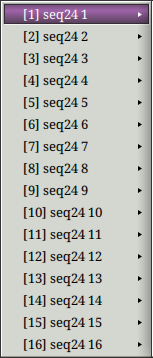
\includegraphics[scale=0.75]{pattern/pattern-menu-midi-bus.png}
   \caption{Existing Pattern, Right-Click Menu, MIDI Output Busses}
   \label{fig:pattern_window_right_click_midi_bus}
\end{figure}

   \textbf{New:}
   \index{new!--bus option}
   Note that another way of specifying the busses is to supply the
   new \texttt{--buss n} option.  This option is currently available
   only from the command line.  It causes \textsl{every} pattern in the MIDI
   file to be allocated to that buss number when loaded, and when a new
   sequence/pattern is created.  This option is
   meant for convenience or testing.  If you save the file, it will then
   have that buss number as part of each track's data, which makes the song
   file just a little less portable.

   For each of these buss items, another pop-up menu allows one
   to specify the MIDI output channel for that buss:

\begin{figure}[H]
   \centering 
   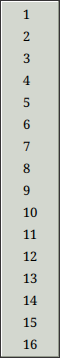
\includegraphics[scale=0.75]{pattern/pattern-menu-midi-bus-numbers.png}
   \caption{Existing Pattern, Right-Click Menu, MIDI Bus Ports}
   \label{fig:pattern_window_right_click_midi_bus_numbers}
\end{figure}

\subsubsection{Pattern Keys and Click}
\label{subsubsec:seq64_patterns_pattern_keys_and_clicks}

   This section recapitulates all the clicks and keys that perform actions
   in the Pattern windows.  Some additional clicks and keys are noted here
   as well.

\paragraph{Pattern Keys}
\label{paragraph:seq64_patterns_pattern_keys}

   \index{keys!hot}
   \index{keys!shortcut}
   Each pattern in the patterns panel can have a hot-key or shortcut-key
   associated with it.

   \index{keys!pattern toggles}
   For each pattern, hitting its assigned shortcut key will
   also toggle its status between muted/unmuted (armed/unarmed).
   Below is the default grid that is
   mapped to the loops/patterns on the screen set.
   This grid can be changed in the Keyboard options tab, and is
   saved in the \textsl{keyboard-control} section of the
   \index{rc file}
   "rc" file.

   \begin{verbatim}
     [ 1   ][ 2   ][ 3   ][ 4   ][ 5   ][ 6   ][ 7   ][ 8   ]
     [ q   ][ w   ][ e   ][ r   ][ t   ][ y   ][ u   ][ i   ]
     [ a   ][ s   ][ d   ][ f   ][ g   ][ h   ][ j   ][ k   ]
     [ z   ][ x   ][ c   ][ v   ][ b   ][ n   ][ m   ][ ,   ]
   \end{verbatim}

   These characters are shown in the lower right corner of each
   pattern, as an aid to memory.
   These hot-keys can be modified.

   \index{keys![}
   \index{keys!decrement set}
   The \texttt{[} and
   \index{keys!]}
   \index{keys!increment set}
   \texttt{]} keys on the keyboard
   switch between sets, either decrementing or incrementing the set number.

   The left and right \texttt{Alt} keys are, by default, set up in the
   \textbf{File / Options / Keyboard / Snapshot 1} and
   \textbf{Snapshot 2} fields to be used as "snapshot" keys.
   Our preference is to use something that does not trigger desktop
   commands, perhaps \texttt{F11} or \texttt{F12}.

   When one of these snapshot keys is pressed, the state of the patterns
   (which ones are armed versus unarmed) is instantly saved.  While the
   snapshot key is held pressed, one can then change the state of the patterns
   (using the keyboard, \textsl{not} the mouse)
   to change how the song plays.  When the snapshot key is released, the
   original saved state of the patterns is restored.

   \index{keys!alt}
   Holding \texttt{Alt} will save the state of playing patterns and restore
   them when \texttt{Alt} is lifted.

   The handling of \texttt{Alt} is often taken over by the window
   manager, so there could be a need to change these items to some other
   keys.  For example, we have Fluxbox set up so that the \texttt{Alt} keys can
   be used for moving or resizing a window.

%  \index{keys!left ctrl alt}
%  Holding \texttt{Left Ctrl} and \texttt{Alt} at the same time will enable
%  one to flip over to new patterns briefly and then flip right back upon
%  lifting \texttt{Alt}.  Not yet sure exactly what this means.

   \index{keys!right ctrl}
   \index{keys!queue}
   \index{queue!temporary}
   Holding \texttt{Right Ctrl}
   will queue a on/off toggle for a 
   sequence when the loop ends. This is the "queue" functionality.
   This means that the change in state of the pattern will not take hold
   immediately, but will kick in when the pattern restarts.
   This pending state is indicated by coloring the central box of the
   pattern grey, as shown in the following figure.

   \textbf{Warning}:  We do not recommend using \texttt{Ctrl} or \texttt{Alt}
   keys for pattern control.  They conflict with application or desktop
   settings.
   The \texttt{Super} key can be used (if not already used by the desktop
   environment).  Also available are some of the function keys, and, if
   available, the keypad keys.  These can be configured in
   \textbf{Options / Keyboard}.

\begin{figure}[H]
   \centering 
   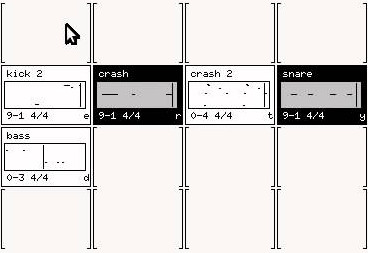
\includegraphics[scale=0.75]{pattern/seq24-queueing-coloration.jpg}
   \caption{Pattern Coloration when Queued}
   \label{fig:seq64_queueing_coloration}
\end{figure}

   Note that queueing can also be used to turn a pattern \textsl{off}
   at the end of a pattern.

   Queue also works for mute/unmute pattern sets ("groups"); in this case,
   every sequence will toggle its status after its individual loop end. 

   Of course, the \texttt{Ctrl} key is used to manage the GUI (e.g.
   \texttt{Ctrl-Q} will unceremoniously quit the application), so one will
   usually want to change this key to something else in the
   \textbf{File / Options / Keyboard / Queue} field.
   The Super key (i.e. the Mod4 or Windows key) is a good candidate to
   replace the right \texttt{Ctrl} key, unless one has (like the author)
   configured the window manager to use the Super key modifier to manipulate
   windows and applications \textsl{(laughter ensues)}.
   However, we have found that one can also use normal keys to enable queueing.
   For example, the minus key or the keypad's slash key can be used, with no
   noticeable flickering due to the keyboard repeat rate.

   \index{keys!replace}
   Note that there is also a "replace" key, which is the left \texttt{Ctrl} key
   by default.  Replacement is a form of muting/unmuting.  When the "replace"
   key is pressed while click a sequence, that sequence is unmuted, and all
   of the other sequences are muted.  Again, this is a very inconvenient
   default, so an alternative key mapping is provided.

   \index{keys!backslash}
   \index{keys!keep queue}
   \index{queue!permanent}
   \index{queue!keep queue}
   Pressing the "keep queue" key (by default, the backslash key)
   \index{rc file}
   assigned in the "rc" file.
   activates permanent queue mode until you use the temporary 
   queue function again pressing \texttt{Right Ctrl}. 
   After pressing the "keep queue" key, individual pattern
   toggles will occur at the end of the current pattern rather than immediately.
   “Keep queue” mode is canceled by pressing the Queue key (right \texttt{Ctrl}).

   This key can be changed in the
   \textbf{File / Options / Keyboard / Keep queue} field.

   There are more keys defined in the \textbf{Keyboard} dialog, and it is
   worth figuring out what they do, if not documented here.
   For a couple of short, but good, tutorials about using arming, queueing,
   and snapshots, see references \cite{wootangent1}
   and \cite{wootangent2}.

\paragraph{Pattern Clicks}
\label{paragraph:seq64_patterns_pattern_Clicks}

   \index{pattern!left click}
   \index{pattern!mute toggle}
   Left-clicking on a pattern-filled box will change its state
   \index{pattern!mute}
   \index{pattern!unmute}
   from muted (white background) to playing (black background) when
   the sequencer is running.

% OBSOLETE:
%
%  \index{pattern!left ctrl left click}
%  \index{keys!left ctrl}
%  Holding down \texttt{Left Ctrl} while selecting a pattern
%  with a left click will mute all other patterns and turn on the selected
%  pattern.

   \index{pattern!left click-drag}
   By clicking and holding the left mouse button on a pattern,
   one can drag it to a new location on the grid.  The box
   will disappear while dragged, and reappear in the new location when
   dropped.  However, note that a pattern cannot be dragged if its
   Pattern Editor window is open.

   \index{pattern!right click}
   Right-clicking a pattern will bring up the appropriate context menus, as
   discussed earlier, depending on whether the pattern box is empty or
   filled.

   \index{pattern!middle click}
   Middle-click does nothing when the mouse rests inside a pattern box.

\subsection{Patterns / Bottom Panel}
\label{subsec:seq64_patterns_panel_bottom}

   The bottom panel of the Patterns window provides way to control the
   overall playback of the song.

\begin{figure}[H]
   \centering 
   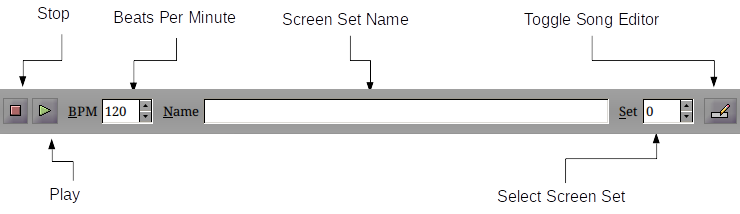
\includegraphics[scale=0.75]{pattern-window-bottom-panel-items.png}
   \caption{Patterns Panel, Bottom Panel Items}
   \label{fig:pattern_window_bottom_panel_items}
\end{figure}

   \begin{enumber}
      \item \textbf{Stop}
      \item \textbf{Play}
      \item \textbf{Pause} (new)
      \item \textbf{BPM}
      \item \textbf{Name}
      \item \textbf{Set}
      \item \textbf{Toggle Song Editor}
   \end{enumber}

   \setcounter{ItemCounter}{0}      % Reset the ItemCounter for this list.

   \itempar{Stop}{pattern!stop}
   The red square button stops the playback of the song and all its patterns.
   It is not clear if it also sends MIDI Off messages on all notes.
   \index{keys!esc (stop)}
   The keystroke for stopping playback is the \texttt{Escape} character.
   It can be changed to \texttt{Space}, so that the space-bar then becomes a
   playback toggle key.

   \itempar{Play}{pattern!Play}
   The green triangular button starts the playback of the whole song.
   \index{keys!space (play)}
   The keystroke for starting playback is the \texttt{Space} character.

   \itempar{Pause}{pattern!Pause}
   \index{new!pause}
   A new feature is that the Play button can be used as a Pause button.
   When the Play button is clicked, the button icon changes to a Pause icon:

\begin{figure}[H]
   \centering 
   
\includegraphics[scale=1.0]{new/stop_pause_buttons.png}
   \caption{Patterns Panel, Pause Button}
   \label{fig:pattern_window_pause_button}
\end{figure}

   Note that a corresponding Pause key (by default, the period) has also been
   defined.  The pause feature can be removed by rebuilding the application
   after configuring with the \texttt{--disable-pause} option.

   \itempar{BPM}{pattern!BPM}
   The spin widget adjusts the "Beats Per Minute" or BPM value.  The
   range of this field is from 20 bpm to 500 bpm, with a default value of
   120 bpm.
   Although this field looks editable, it is not.  Most keystrokes
   that are entered actually toggle one of the pattern boxes.
   However, the following keys can also modify the BPM in small increments:
   \index{keys!semicolon} The \texttt{semicolon} reduces the BPM;
   \index{keys!apostrophe} The \texttt{apostrophe} increases the BPM.
   Also, if one right-clicks on the Up button, the BPM advances to its largest
   supported value, and if one right-clicks on the Down button, the BPM
   advances to its lowest value.  The legal range is from 1 to 500 BPM.

   \itempar{Name}{pattern!set name}
   Each of the 32 available screen sets can be given a name by entering it
   into this field.

   \textbf{Bug:}
   \index{bugs!set name has side-effect}
   While one is typing in the name of the set in this field, the keystrokes
   will affect the panel window, causing playback to start and pattern
   boxes to be toggled!

   \itempar{Set}{pattern!set number}
   This spin widget selects the current screen set.  The values in this
   field range from 0 to 31, and default to 0.
   Although this field looks editable, it is not.

   \textbf{Bug:}
   \index{bugs!set number has side-effect}
   While one is typing in the number of the set in this field, the keystrokes
   will affect the panel window as well.

   \itempar{Toggle Song Editor}{pattern!toggle song editor}
   Pressing this button toggles the presence on-screen of the Song
   Editor.

%-------------------------------------------------------------------------------
% vim: ts=3 sw=3 et ft=tex
%-------------------------------------------------------------------------------
